\chapter{Análise de Dados e Resultados}

Este capítulo cumpre o objetivo de analisar os enunciados das notícias econômicas sob a ótica do processamento de linguagem natural e suas possíveis relações com as variáveis econômicas. Em sua primeira seção, será acompanhado a construção dos Índices de Sentimento Econômico ao longo do tempo. Após essa etapa, na segunda parte do capítulo iremos avaliá-los sob a perspectiva econométrica e então avaliação dos seus resultados. Os códigos utilizados neste capítulo podem ser encontrados em <\url{https://github.com/santluan/monografiaUFF}>.

\section{Índices de Sentimento de Notícias}

Os dados para construção do índice foram extraídos a partir dos enunciados das notícias econômicas do veículo de mídia \cite{folha-mercado} durante o período de 2011 a 2022, com auxílio da linguagem \textit{Python}. Para este procedimento foram utilizados métodos de \textit{web scraping} das postagens do @folha\_mercado no \textit{Twitter} contendo apenas os enunciados das notícias de mercado. Após isso, foi feita tradução para inglês dos mesmos pois todos os léxicos utilizados nesse estudo são deste idioma. Na Figura \ref{fig: wordcloud} podemos observar a nuvem de palavras com os termos de maior frequência. 

\begin{figure}[htp!]
\centering
\caption{Nuvem de palavras gerada a partir dos enunciados do jornal Folha Mercado}
\label{fig: wordcloud}
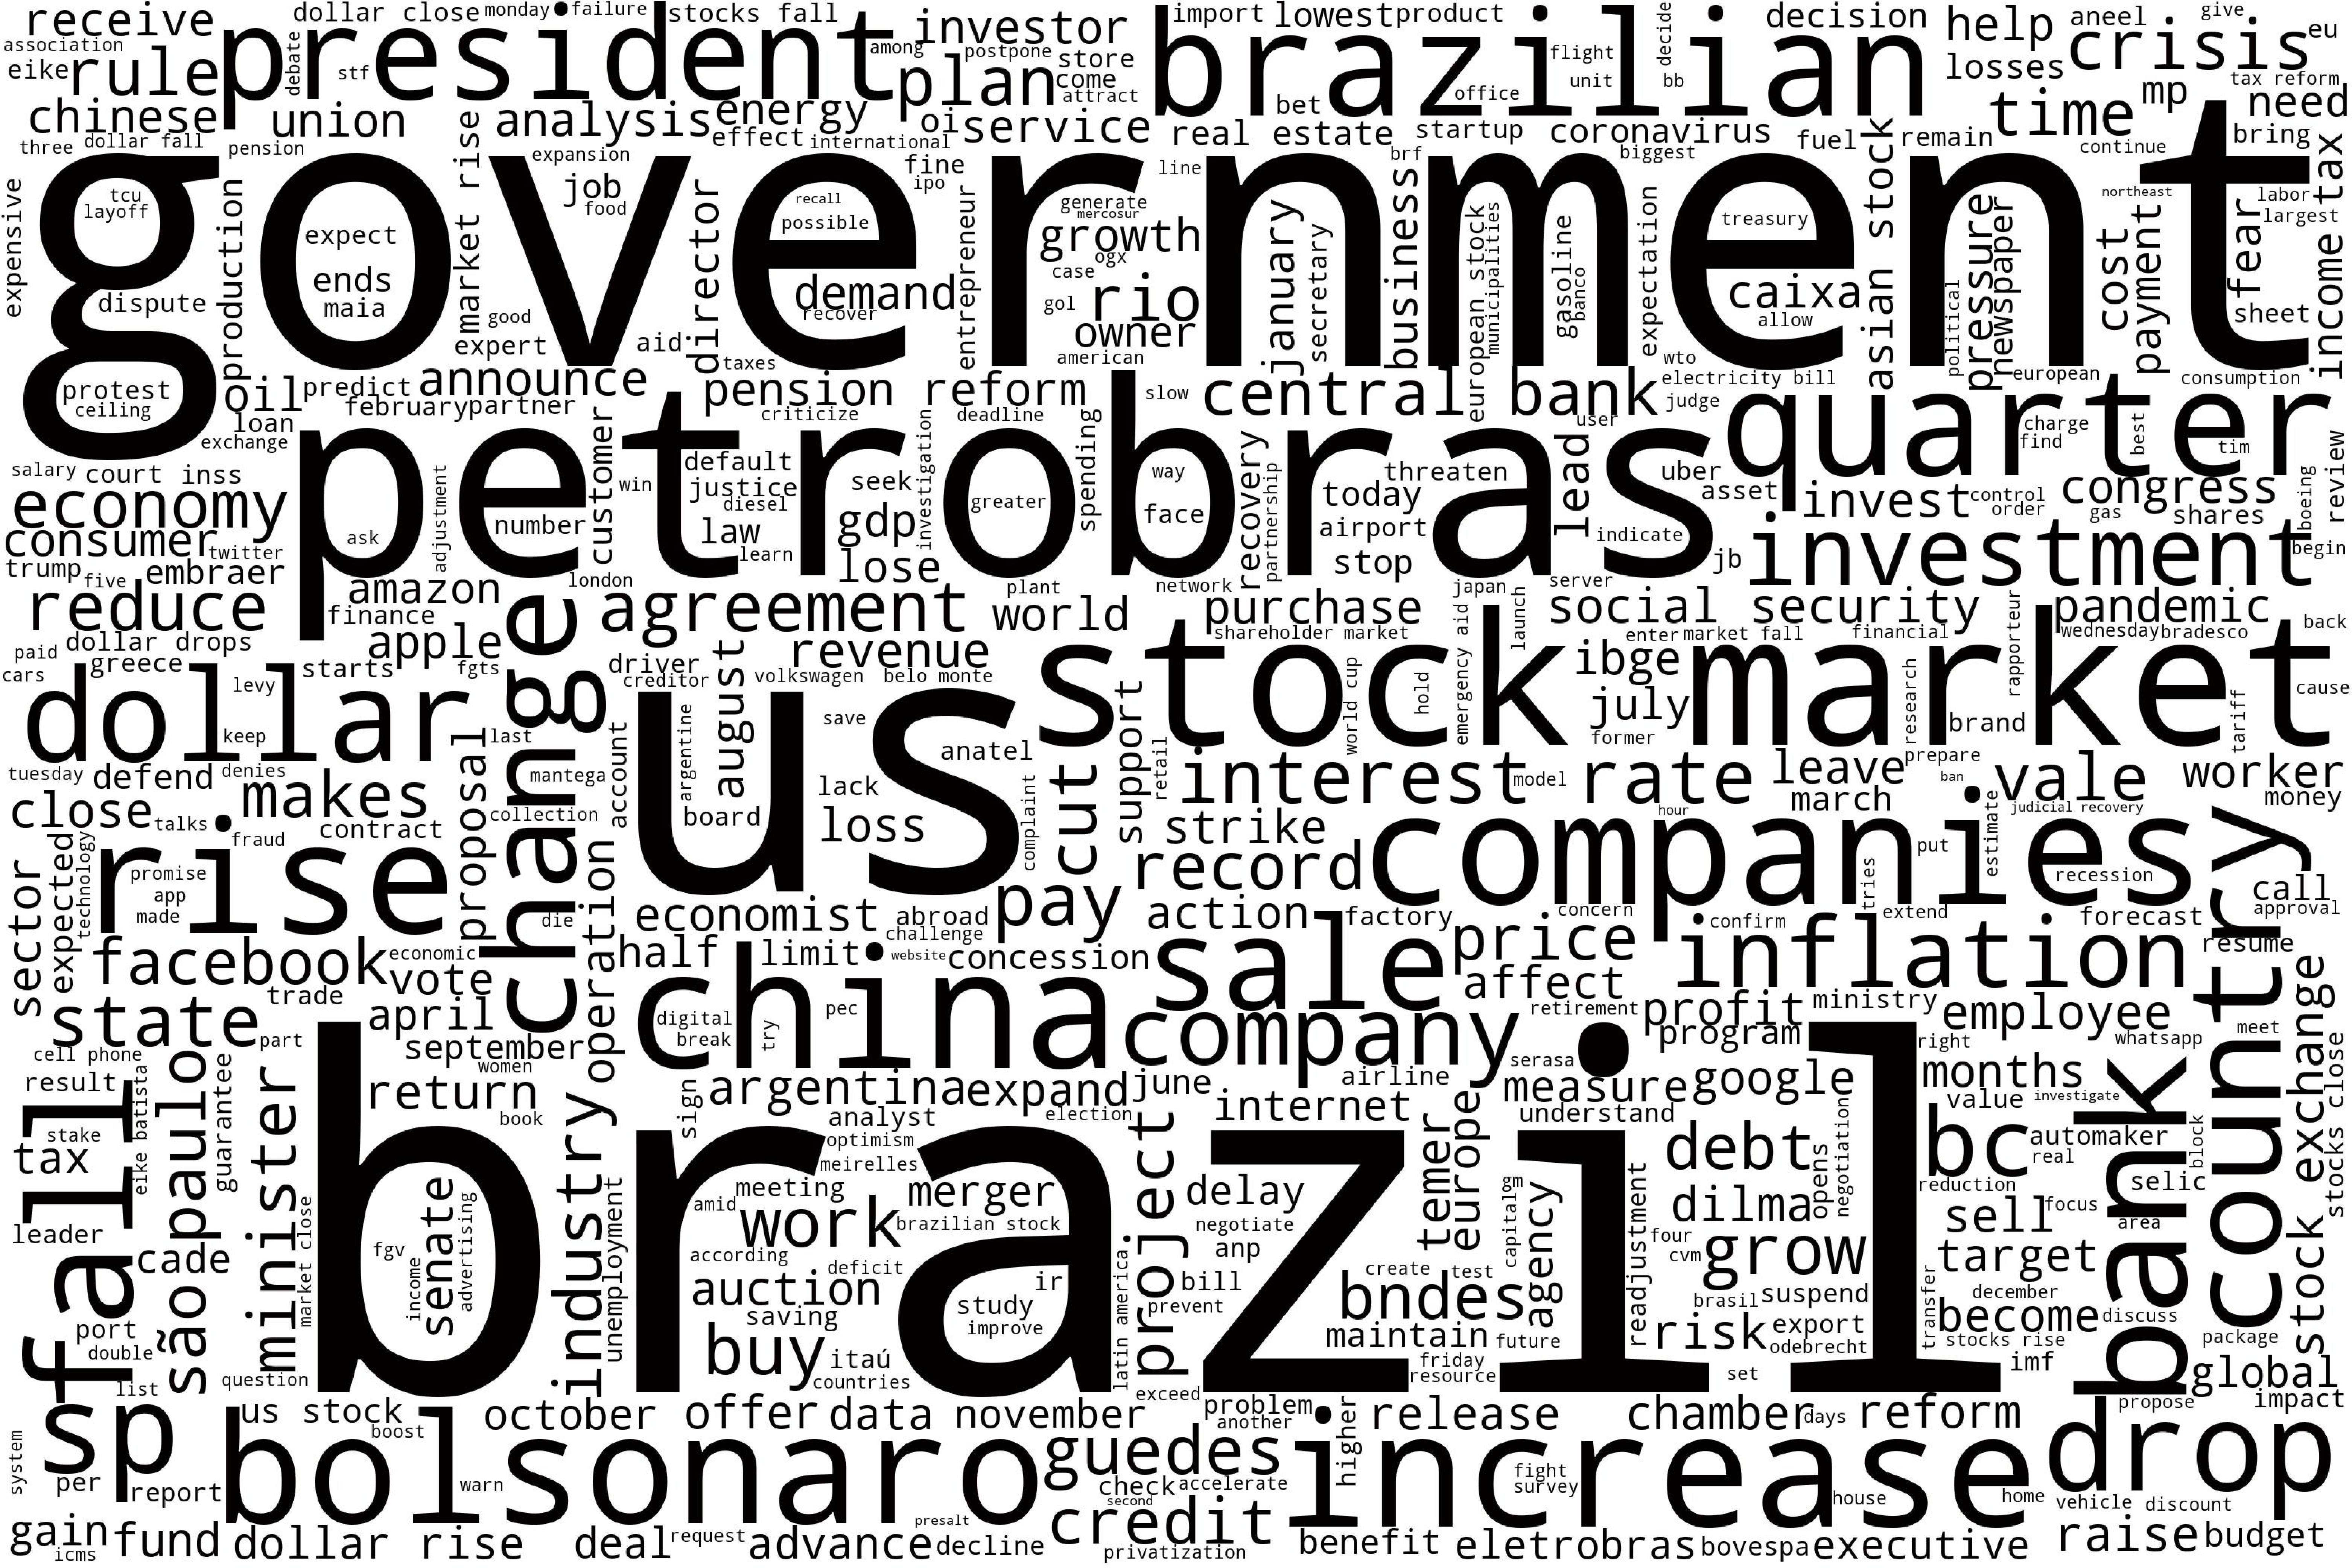
\includegraphics[width=0.8\textwidth]{imagens/wordcloud_tweets.pdf}
\caption*{Fonte : Elaboração Própria}
\end{figure}

Dentre as palavras mais utilizadas, é perceptível termos relacionados ao mercado, como mercado de ações, inflação, taxa de juros, Petrobras, crise, assim como palavras com relação ao governo e política, com menções ao Presidente em exercício e anteriores a ele. Além destes, também é visto palavras comuns ao noticiário econômico financeiro, tais como queda, alta, aumento, elevação, entre outras. Podemos observar a frequência das principais palavras do corpus na Tabela \ref{tab:contgeral}.

\begin{table}[!h]
\centering
\caption{Palavras com maior frequência nas manchetes do Folha Mercado}
\begin{tabular}{ll|ll|ll}
\hline
Palavra     & n     & Palavra   & n    & Palavra   & n    \\ \hline
government  & 4574  & petrobras & 2589 & oil       & 1555 \\
market      & 3330  & rises     & 1749 & president & 1498 \\
us          & 3085  & companies & 1687 & bank      & 1490 \\
brazil      & 3050  & tax       & 1672 & reform    & 1384 \\
stock       & 2968  & interest  & 1574 & bolsonaro & 1326 \\ \hline
\end{tabular} \label{tab:contgeral}
\end{table}

\subsection{Índice de Sentimento utilizando VADER - ISV}

A partir desse corpus de texto ainda não é possível inferir o nível de incerteza ou otimismo do mercado e de seus agentes quanto à economia. Para isso, iremos utilizar o algoritmo VADER, idealizado por \citeonline{vader}, e o dicionário LM-SA-2020, desenvolvido por \citeonline{lmsa2020}, para compreender o sentimento expresso nos dados textuais das notícias econômicas e financeiras. Tais técnicas irão auxiliar na geração do índice de sentimento e, consequentemente, compreender o nível de otimismo ou pessimismo geral dos meios de mídia informacional.

Para construção dos índices, foi utilizado a linguagem de programação \textit{Python} (\citeonline{python3}) pela sua grande capacidade de processamento, sintaxe simples, facilidade na implementação e pela sua ampla utilização no meio acadêmico, especialmente entre pesquisadores e entusiastas da NLP. Tendo isso em vista, para o índice VADER foi usado o pacote \textit{nltk} (\textit{Natural Language Toolkit} \citeonline{nltk}) do \textit{Python} que abrange técnicas do campo de processamento de linguagem natural. Vale lembrar que o VADER é idealmente criado para análise de texto de mídias sociais, tais como \textit{Twitter} e \textit{Facebook}. Entretanto, ele é uma das ferramentas mais completas para compreensão de sentimentos em texto e, por este motivo, é escolhido nesse estudo para criação de um dos índices.

Para construção do índice VADER, contabilizado para cada enunciado de notícia $i$, é quantificado o número de palavras classificadas como positivas ($Wp$) e negativas ($Wn$) de um total de palavras $W_i$. Assim, o índice VADER pode ser representado pela diferença entre $Wp_i$ e $Wn_i$ em relação ao total $W_i$, isto é
\begin{align} \label{indicevader}
    ISV_i = \frac{Wp_i - Wn_i}{W_i} \quad ,
\end{align}

\noindent dessa maneira, o índice VADER (ISV) denota a razão de polaridade do texto, ou seja, da notícia em questão. Apesar do VADER possuir outras métricas para estudo, foi optado pelo índice dos enunciados para medir o nível de incerteza e pessismismo das mídias e, portanto, da economia brasileira.

É importante salientar que o índice foi construído com periodicidade mensal, a partir da média dos resultados obtidos para cada notícia no período em questão. Foi escolhido seguir dessa maneira para efeito de comparação com as demais séries de dados.

\begin{figure}[!h]
    \centering
    \caption{Índice de Sentimento mensal VADER}
    \label{fig: ISV}
    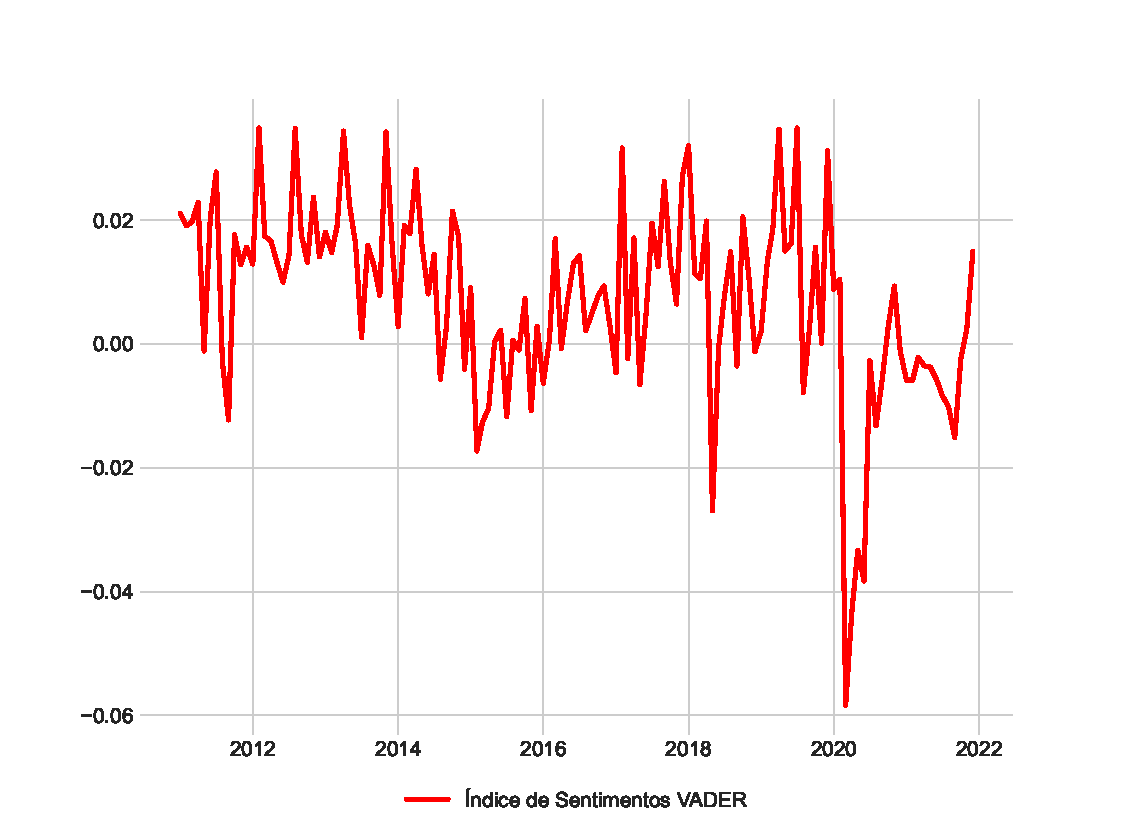
\includegraphics[width=0.85\textwidth]{imagens/isv.pdf}
    \caption*{Fonte : Elaboração Própria}
\end{figure}

Como demonstrado na Figura \ref{fig: ISV}, é notável mencionar que o índice de sentimento possui alta variabilidade, adotando uma tendência média temporal oscilante, com períodos de sentimento positivo e negativo. Além disso, percebe-se altos picos e quedas no seu nível, sendo os mais notáveis entre os períodos de 2014-2016 durante a recessão econômica em território brasileiro, onde podemos notar um tendência de queda durante esse período, inclusive com sentimentos negativos. Outro exemplo desse comportamento é durante o ano de 2020 com a incidência da pandemia de COVID-19, no qual é possível ver uma queda significante do índice e se mantendo num patamar predominante negativo no restante da série. Ao capturar tais acontecimentos, o índice VADER corrobora a ideia de indicador do sentimento das notícias econômicas e, portanto, da economia em geral.

\begin{figure}[!h]
    \centering
    \caption{Gráfico de Densidade para o Índice de Sentimentos VADER}
    \label{fig: ISV density}
    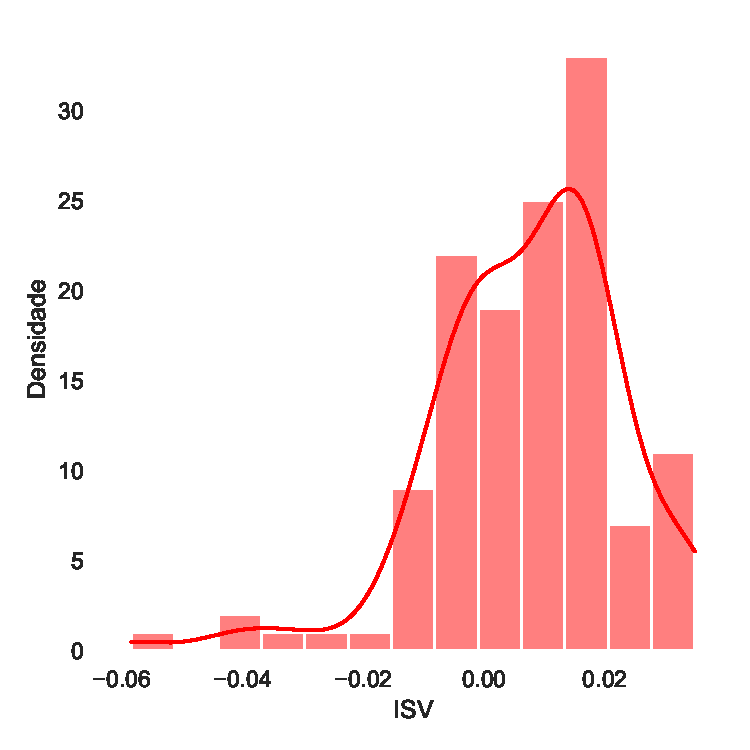
\includegraphics[width=0.55\textwidth]{imagens/isv_densityplot.pdf}
    \caption*{Fonte: Elaboração Própria}
\end{figure}

Na Figura \ref{fig: ISV density} podemos observar a densidade para os dados do índice VADER. Apesar de seus resultados variarem bastante ao londo da série, indo de $-0,06$ à $0,04$, percebe-se que seus valores são predominantemente positivos, com uma densidade positiva centralizada entre $0,0$ e $0,02$. 

\subsection{Índice de Sentimento utilizando LM-SA-2020 - ISL}

Em busca de ferramentais que melhor se adequem ao campo econômico, foi construído o segundo Índice de Sentimentos a partir do dicionário LM-SA-2020. Este dicionário é originalmente idealizado por \citeonline{loughran2011liability} a partir da análise textual de reports financeiros e atualizado por \citeonline{lmsa2020} com termos mais comuns aos mercados emergentes e subdesenvolvidos. 

%Esta atualização cumpre o dever de adaptar a realidade do dicionário a uma maior gama de mercados e assim melhorar seu desempenho na análise de texto econômico. Os resultados encontrados pelos autores demonstram uma melhora significativa nos seus modelos e corroboram a atualização do dicionário para uma dimensão maior da realidade dos mercados. 

Para o índice LM, é implementado código para busca da palavra no dicionário e identificação da mesma entre positivo e negativo. Logo após identificação, é realizado cálculo para as suas frequências relativas, dentro do seu corpus de texto, e então dimensionamento no texto. Por fim, os procedimentos para desenvolvimento final do índice seguem a mesma metodologia do Índice VADER abordados anteriormente.

Na Figura \ref{fig: ISL} nota-se uma similaridade entre os índices ISV e ISL, sendo uma série com alta variação. Entretanto, podemos observar também que, para o período especificado, o índice possui um perfil negativo ao longo da série, com tendência média temporal negativa. Isto é, do ponto de vista econômico, o ISL indica o sentimento das notícias marcado pela negatividade, diferentemente do ISV que aponta períodos negativos intercalados de períodos de sentimento positivo. Além disso, é notável os períodos de queda acentuada dos seus níveis durante a recessão econômica e pandemia, semelhante aos vistos no VADER.

\begin{figure}[!h]
    \centering
    \caption{Índice de Sentimento mensal LM-SA}
    \label{fig: ISL}
    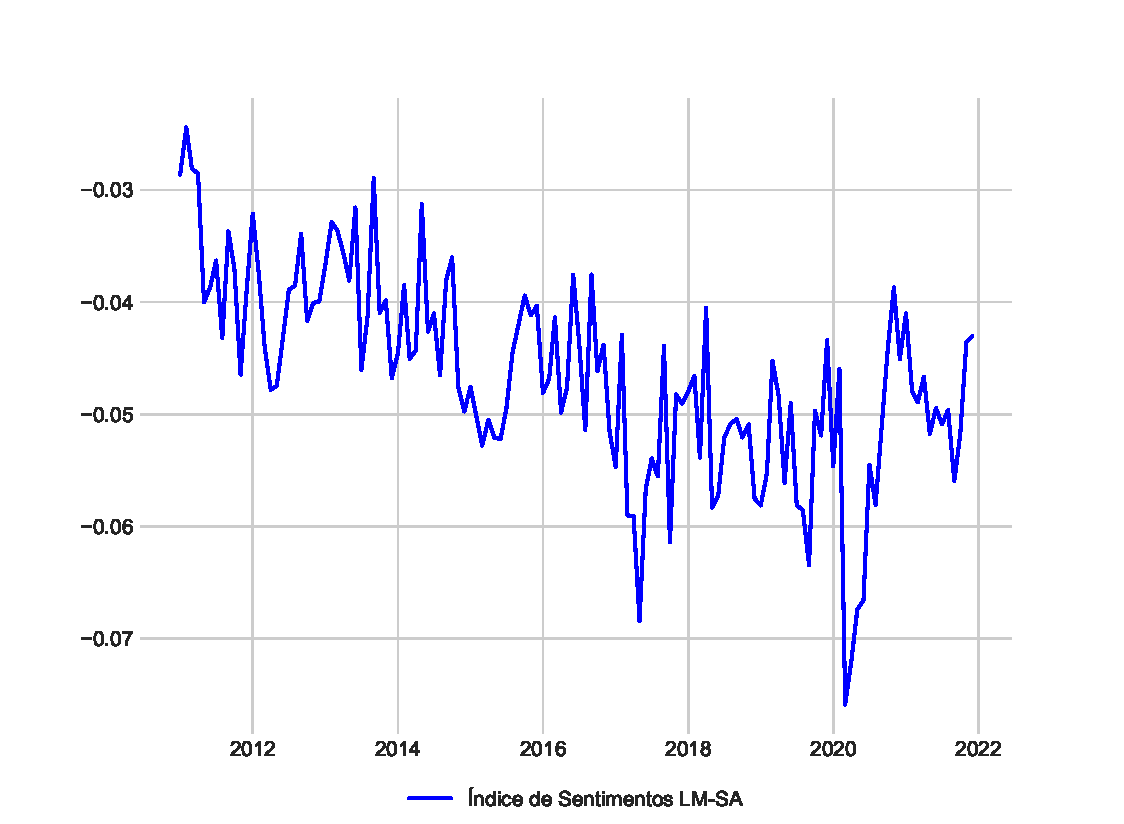
\includegraphics[width=0.85\textwidth]{imagens/isl.pdf}
    \caption*{Fonte : Elaboração Própria}
\end{figure}


A Figura \ref{fig: ISL density} salienta a alta variabilidade do índice, com uma densidade negativa. Tal comportamento se deve provavelmente pela metodologia seguida por cada dicionário dos índices, visto que o primeiro é um algoritmo generalista para análise de sentimentos, enquanto que o segundo possui fundamentação econômica.

\begin{figure}[!h]
    \centering
    \caption{Gráfico de Densidade para o Índice de Sentimentos LM-SA}
    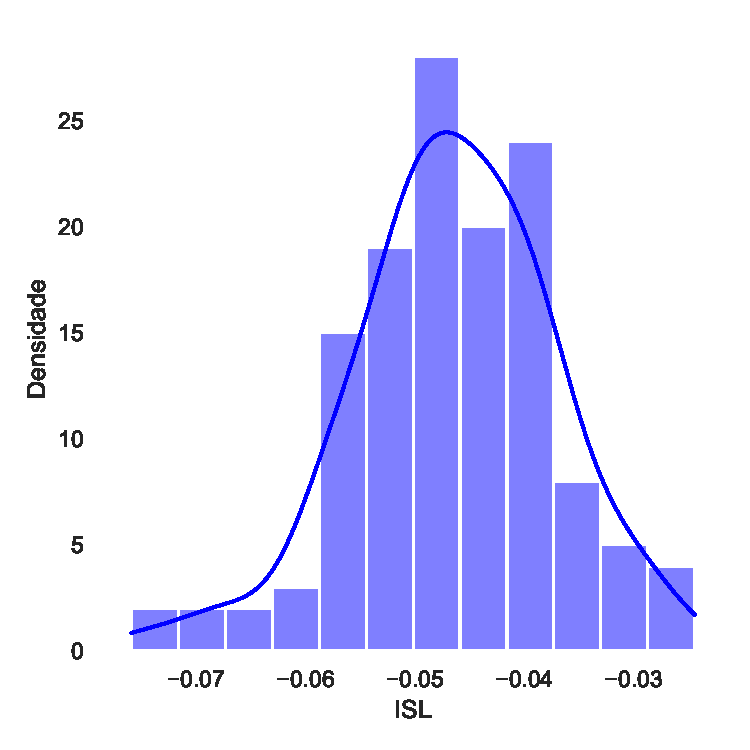
\includegraphics[width=0.55\textwidth]{imagens/isl_densityplot.pdf}
    \caption*{Fonte: Elaboração Própria}
    \label{fig: ISL density}
\end{figure}

Para uma melhor visão, a Figura \ref{fig: vaderxlmsa} demonstra a evolução das séries para o período estudado. Para este processo, os dados foram normalizados para termos uma comparabilidade entre os índices. É possível observarmos semelhanças entre as duas séries, principalmente nos períodos de maior ápice e queda nos seus níveis. Além disso, é valido notar os comportamentos conjuntos durante os períodos mais conturbados para a economia nos últimos anos, como mencionados anteriormente.

\begin{figure}[!h]
    \centering
    \caption{Evolução temporal dos índices ISV e ISL}
    \label{fig: vaderxlmsa}
    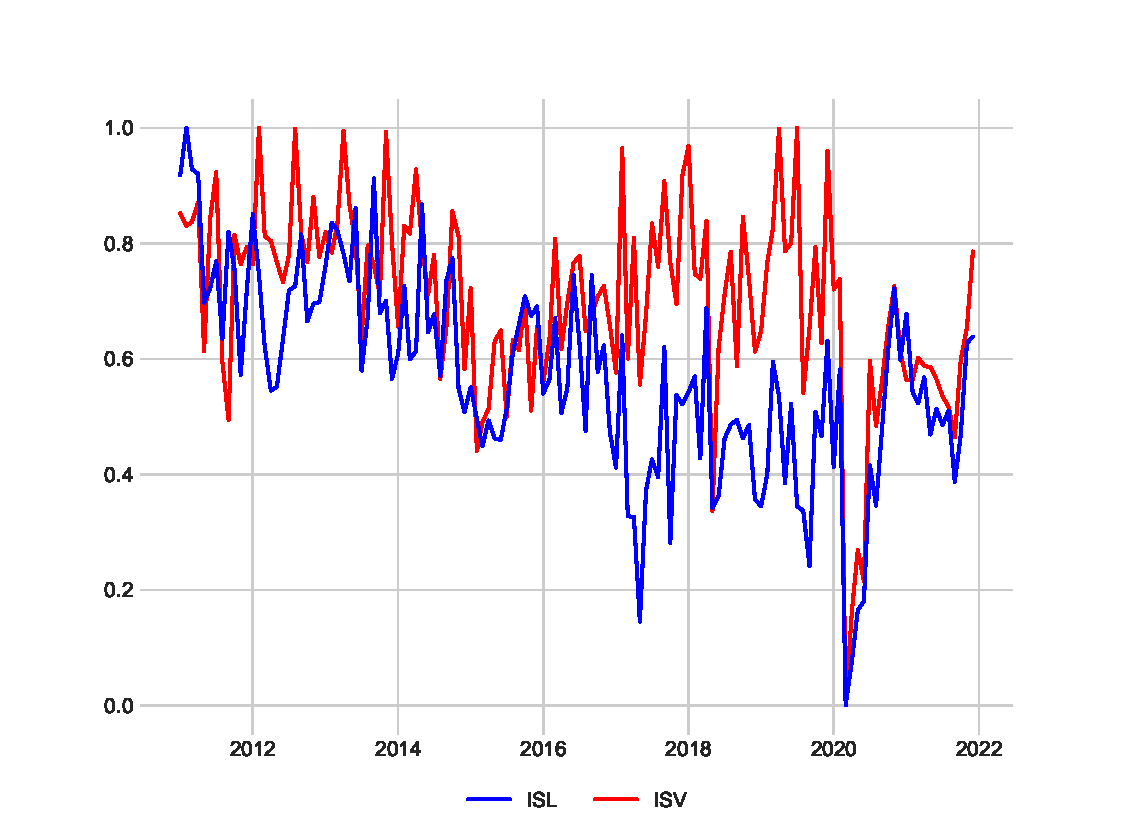
\includegraphics[width=0.8\textwidth]{imagens/isv_isl.pdf}
    \caption*{Fonte : Elaboração Própria}
\end{figure}

Por fim, quando vistas conjuntamente, é percebido como as duas diferenciam-se no nível mas não em sua variação. Enquanto o ISV tem comportamento predominante positivo ao longo do tempo, o ISL, em contrapartida, apresenta valores negativos em toda sua séria. Porém, vemos como as duas possuem caminhos semelhantes em períodos de maior instabilidade econômica e política no país.

%Esse resultado pode ser visualizado comparativamente na Figura \ref{fig: densitytotal} onde vemos as densidades dos índices um contra o outro.

%\begin{figure}[!h]
%    \centering
%    \caption{Densidades para ISV e ISL}
%    \includegraphics[width=0.4\textwidth]{imagens/vader_lm_densityplot.pdf}
%    \caption*{Fonte: Elaboração Própria}
%    \label{fig: densitytotal}
%\end{figure}

%As duas séries possuem alta correlação, com um $R$ igual a 0,5776, o que demonstra como as séries tendem a se comportar semelhantemente ao longo do tempo.


\section{Testes Econométricos}

Essa segunda parte irá acompanhar os índices sob a ótica econômica e econométrica a saber sua relevância para previsão e impacto nas demais séries econômicas.

\subsection{Séries Econômicas}

Na Tabela \ref{tab: variaveis}, apresentamos as séries econômicas que iremos utilizar neste estudo, além da sua fonte e código da série a qual se referencia. Todas elas foram extraídas do Sistema de Gerenciador de Séries Temporais do Banco Central do Brasil, podendo ser encontrado em: <\url{https://www3.bcb.gov.br/sgspub}>. Além destas séries, optou-se também pela medição do hiato do produto pela teoria do Filtro de \citeonline{hp-filter} como forma de suavizar as oscilações associadas aos ciclos econômicos. E, por último, foi extraído a série do índice BOVESPA pelo pacote \textit{yfinance} (\citeonline{yfinance}) do \textit{Python} e medido os retornos mensais para o índice.

\begin{table}[!h]
\caption{Variáveis Econômicas}
\centering
\begin{tabular}{llllc}
\hline
Dados  & Fonte & Série \\
\hline
IBC-Br & BCB   & 24364 \\
IPCA   & BCB   & 433   \\
Selic  & BCB   & 432   \\
Índice BOVESPA & B3 & -\\
\hline
\end{tabular} \label{tab: variaveis}
\end{table}

Na Figura \ref{fig: econ_plots} podemos ver as séries econômicas separadamente e identificar como elas agiram nos últimos anos. Para o IBC-Br, vemos que a atividade econômica teve queda pós-recessão e não retornou ao seu patamar anterior. Enquanto IPCA teve grande variação nos preços nos últimos anos, período esse marcado pela alta inflação. A taxa de juros SELIC também passou por longos períodos de alta e baixa nos seus níveis. Por último, é possível observar a série dos retornos com alta variação, sendo destaque para o ano de 2020 com queda acentuada por conta da pandemia.

\begin{figure}[!h]
    \centering
    \caption{Séries Econômicas ao longo do tempo}
    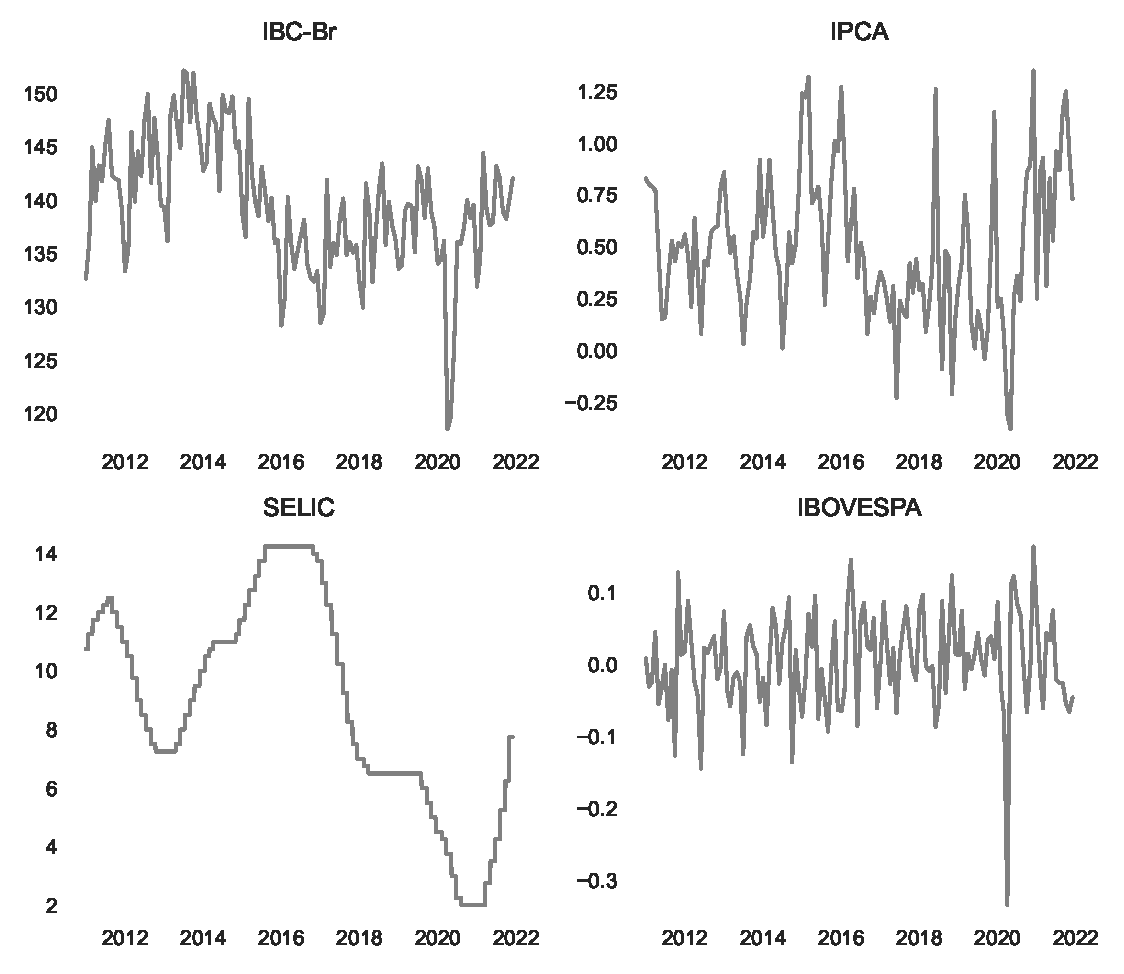
\includegraphics[width=0.55\textwidth]{imagens/econ_plots.pdf}
    \label{fig: econ_plots}
    \caption*{Fonte: BCB e B3. Elaboração Própria.}
\end{figure}

\subsection{Teste de Raíz Unitária}

Seguindo a literatura de séries temporais, é preciso verificar a natureza das variáveis antes de iniciarmos a modelagem dos dados. Para isto, iremos aplicar os testes de estacionariedade mais comuns, sendo eles o teste Dickey-Fuller Aumentado (ADF) e Phillips-Perron (PP) pra checar a presença de raiz unitária nos dados. Para esta tarefa foi escolhido o pacote \textit{aTSA} \cite{aTSA} do R \cite{R} que detém ferramentas para análise de séries temporais, inclusive as da nossa finalidade. Com os testes aplicados para todas as séries, os resultados podem ser vistos nas Tabelas \ref{ADFtest} e \ref{PPtest} a seguir:

\begin{table}[!h]
    \centering
    \caption{Teste de Raiz Unitária: Dickey-Fuller Aumentado}
    \begin{tabular}{llllc}
    \hline
Variáveis & ADF (-) & ADF (C) & ADF (CT) & Lag \\
    \hline
ISV       & -6.0408*** & -6.8393*** & -7.5880*** & 0 \\
ISL       & -0.7492    & -5.2260*** & -6.7830*** & 0 \\
IBC-Br    & -0.0405    & -2.2058    & -2.5468    & 0 \\
Hiato     & -3.7220*** & -3.7072*** & -3.6917**  & 0 \\
IPCA      & -3.1482*** & -5.8397*** & -5.8091*** & 0 \\
Selic     & -1.0038    & -3.1072**  & -2.7798    & 3 \\
IBOVESPA  & -10.2413***& -10.2553***& -10.2860***& 0 \\
D(IBC-Br) & -9.1266*** & -9.0912*** & -9.0584*** & 0 \\
D(Selic)  & -7.1436*** & -7.1419*** & -7.1267*** & 0 \\
    \hline
    \end{tabular} \label{ADFtest}
    \fonte{Elaboração Própria.}
\nota{Rejeita-se a hipótese nula a nível de: * 10\%; ** 5\%; *** 1\%.}
\end{table}

A Tabela \ref{ADFtest} dispõe o teste ADF nas suas três formas, sendo: primeira coluna os resultados sem a presença de constante e tendência (-); segunda coluna com constante (C) e, por último, a presença de ambas (CT). O mesmo raciocínio segue para o teste PP. Diante disso, tendo em vista os resultados, vemos que o ISV rejeita a presença de raiz unitária em todos os cenários, enquanto que o ISL rejeita a hipótese apenas para os cenários com constante e tendência. Os mesmos resultados foram encontrados para o IPCA, Hiato e IBOVESPA, demonstrando que as séries também rejeitam a presença de raíz unitária. As demais séries, IBC-Br e Selic, não apresentaram estacionariedade em nenhum cenário, somente após a primeira diferença que vemos a rejeição da hipótese nula.

\begin{table}[!h]
    \centering
    \caption{Teste de Raiz Unitária: Phillips-Perron}
    \begin{tabular}{llllc}
    \hline
Variáveis & PP (-) & PP (C) & PP (CT) & Lag \\
    \hline
ISV       & -6.0930*** & -7.0061*** & -7.7808*** & 4 \\
ISL       & -0.3273    & -5.0446*** & -6.8785*** & 4 \\
IBC-Br    & -0.0430    & -2.3727    & -2.7976    & 4 \\
Hiato     & -4.0455*** & -4.0319*** & -4.0177*** & 4 \\
IPCA      & -2.7906*** & -5.9139*** & -5.8835*** & 4 \\
Selic     & -0.7768    & -1.1103    & -1.2771    & 4 \\
IBOVESPA  & -10.1821***& -10.2021***& -10.2452***& 4 \\
D(IBC-Br) & -8.9426*** & -8.9023*** & -8.8648*** & 4 \\
D(Selic)  & -7.5156*** & -7.5134*** & -7.4975*** & 4 \\
    \hline
    \end{tabular} \label{PPtest}
    \fonte{Elaboração Própria.}
\nota{Rejeita-se a hipótese nula a nível de: * 10\%; ** 5\%; *** 1\%.}
\end{table}

Ao observarmos a Tabela \ref{PPtest}, vemos que seus resultados se assemelham aos do teste ADF, confirmando que as séries dos índices, do IPCA, Hiato e IBOVESPA são estacionárias. Quanto à SELIC e IBC-Br, nesse caso, prefere-se utilizar suas séries em diferença.

\subsection{Escolha do modelo adequado}

Dada a imensa quantidade de modelos disponíveis em séries temporais, a escolha do mais adequado é crucial para garantir resultados não-viesados. Como visto na Figura \ref{fig: select_model} os autores \citeonline{method-select} demonstram o método para seleção do modelo adequado tendo em vista a natureza das variáveis.

\begin{figure}[!h]
    \centering
    \caption{Método de seleção para Séries Temporais}
    \label{fig: select_model}
    \includegraphics[width=0.7\textwidth]{imagens/method_selection.png}
    \caption*{Fonte: \cite{method-select}}
\end{figure}

As séries selecionadas para o modelo foram as dos índices ISV e ISL, IPCA, Hiato,  IBOVESPA e Selic em diferença, por serem estacionários e darem mais robustez ao modelo. Dessa forma, seguindo a método de seleção idealizado da Figura \ref{fig: select_model} foi escolhido prosseguir com o modelo Vetorial Autoregressivo (VAR), por se tratar de um modelo multivariado que melhor representa o comportamento conjunto das séries de dados e em estacionariedade. Além disso, esse modelo trabalha com a dificuldade enfrentada em séries de natureza endógena, que é o caso deste trabalho. Por lidar com estas dificuldades e também pelas vantagens apresentadas, o modelo VAR é o melhor para realizar a pesquisa desta monografia. Dessa maneira, no contexto da representação da técnica VAR e de sua função de resposta impulso postuladas teoricamente nas Equações (\ref{var-reduzido}) e (\ref{VAR-FIR}), consideraremos dois modelos diferenciados somente pela componente do índice de sentimentos. Assim sendo, o Modelo 1 contém o índice ISV no vetor $x_{1t}$, e Modelo 2 o índice ISL no vetor $x_{2t}$; isto é, simbolicamente representados como:

\begin{align}
    x_{1t} = 
    \begin{bmatrix}
    ISV \\ Hiato \\ IPCA \\ D(Selic) \\ IBOVESPA
    \end{bmatrix}
\quad , \quad
    x_{2t} = 
    \begin{bmatrix}
    ISL \\ Hiato \\ IPCA \\ D(Selic) \\ IBOVESPA
    \end{bmatrix}
\quad .
\end{align}

\subsection{Função de Resposta Impulso}

%Tendo realizado os testes de raiz unitária e escolha do modelo adequado, partiremos em busca de entender o papel efetivo dos índices de sentimentos em mensurar o nível de otimismo ou pessimismo dos agentes econômicos, além de, também, compreender a sua influência sobre a economia em geral. Diante disso, 
Nesta seção final iremos observar o impacto dos índices baseados em sentimento sobre as demais séries econômicas. Em outras palavras, iremos observar o comportamento das séries diante de um choque positivo causado pelos índices.

Para isto, iremos começar com a estimação de um modelo VAR e então mensurar as funções de resposta impulso para cada índice. A escolha da ordem de integração do modelo VAR se deu pela consulta dos critérios de informação \citeonline{akaike-criterion}, \citeonline{schwarz} e \citeonline{hanna-quinn}. Com os resultados em mãos, foi escolhido prosseguir com a estimação de um VAR(3) para ambos os índices. Vale recordar que a Função de Resposta Impulso demonstra como as séries do modelo reagem a um dado choque positivo sobre uma série. Neste caso, irei primeiramente causar um choque no índice VADER (ISV) e verificar seus comportamentos sobre as demais séries. É importanto mencionar que, para este trabalho, estamos utilizando um intervalo de confiança de 95\% para as resultados da função.

\begin{figure}[!h]
    \centering
    \caption{Função de Resposta ao Impulso para o Modelo 1 - ISV}
    \label{fig: irf_isv}
    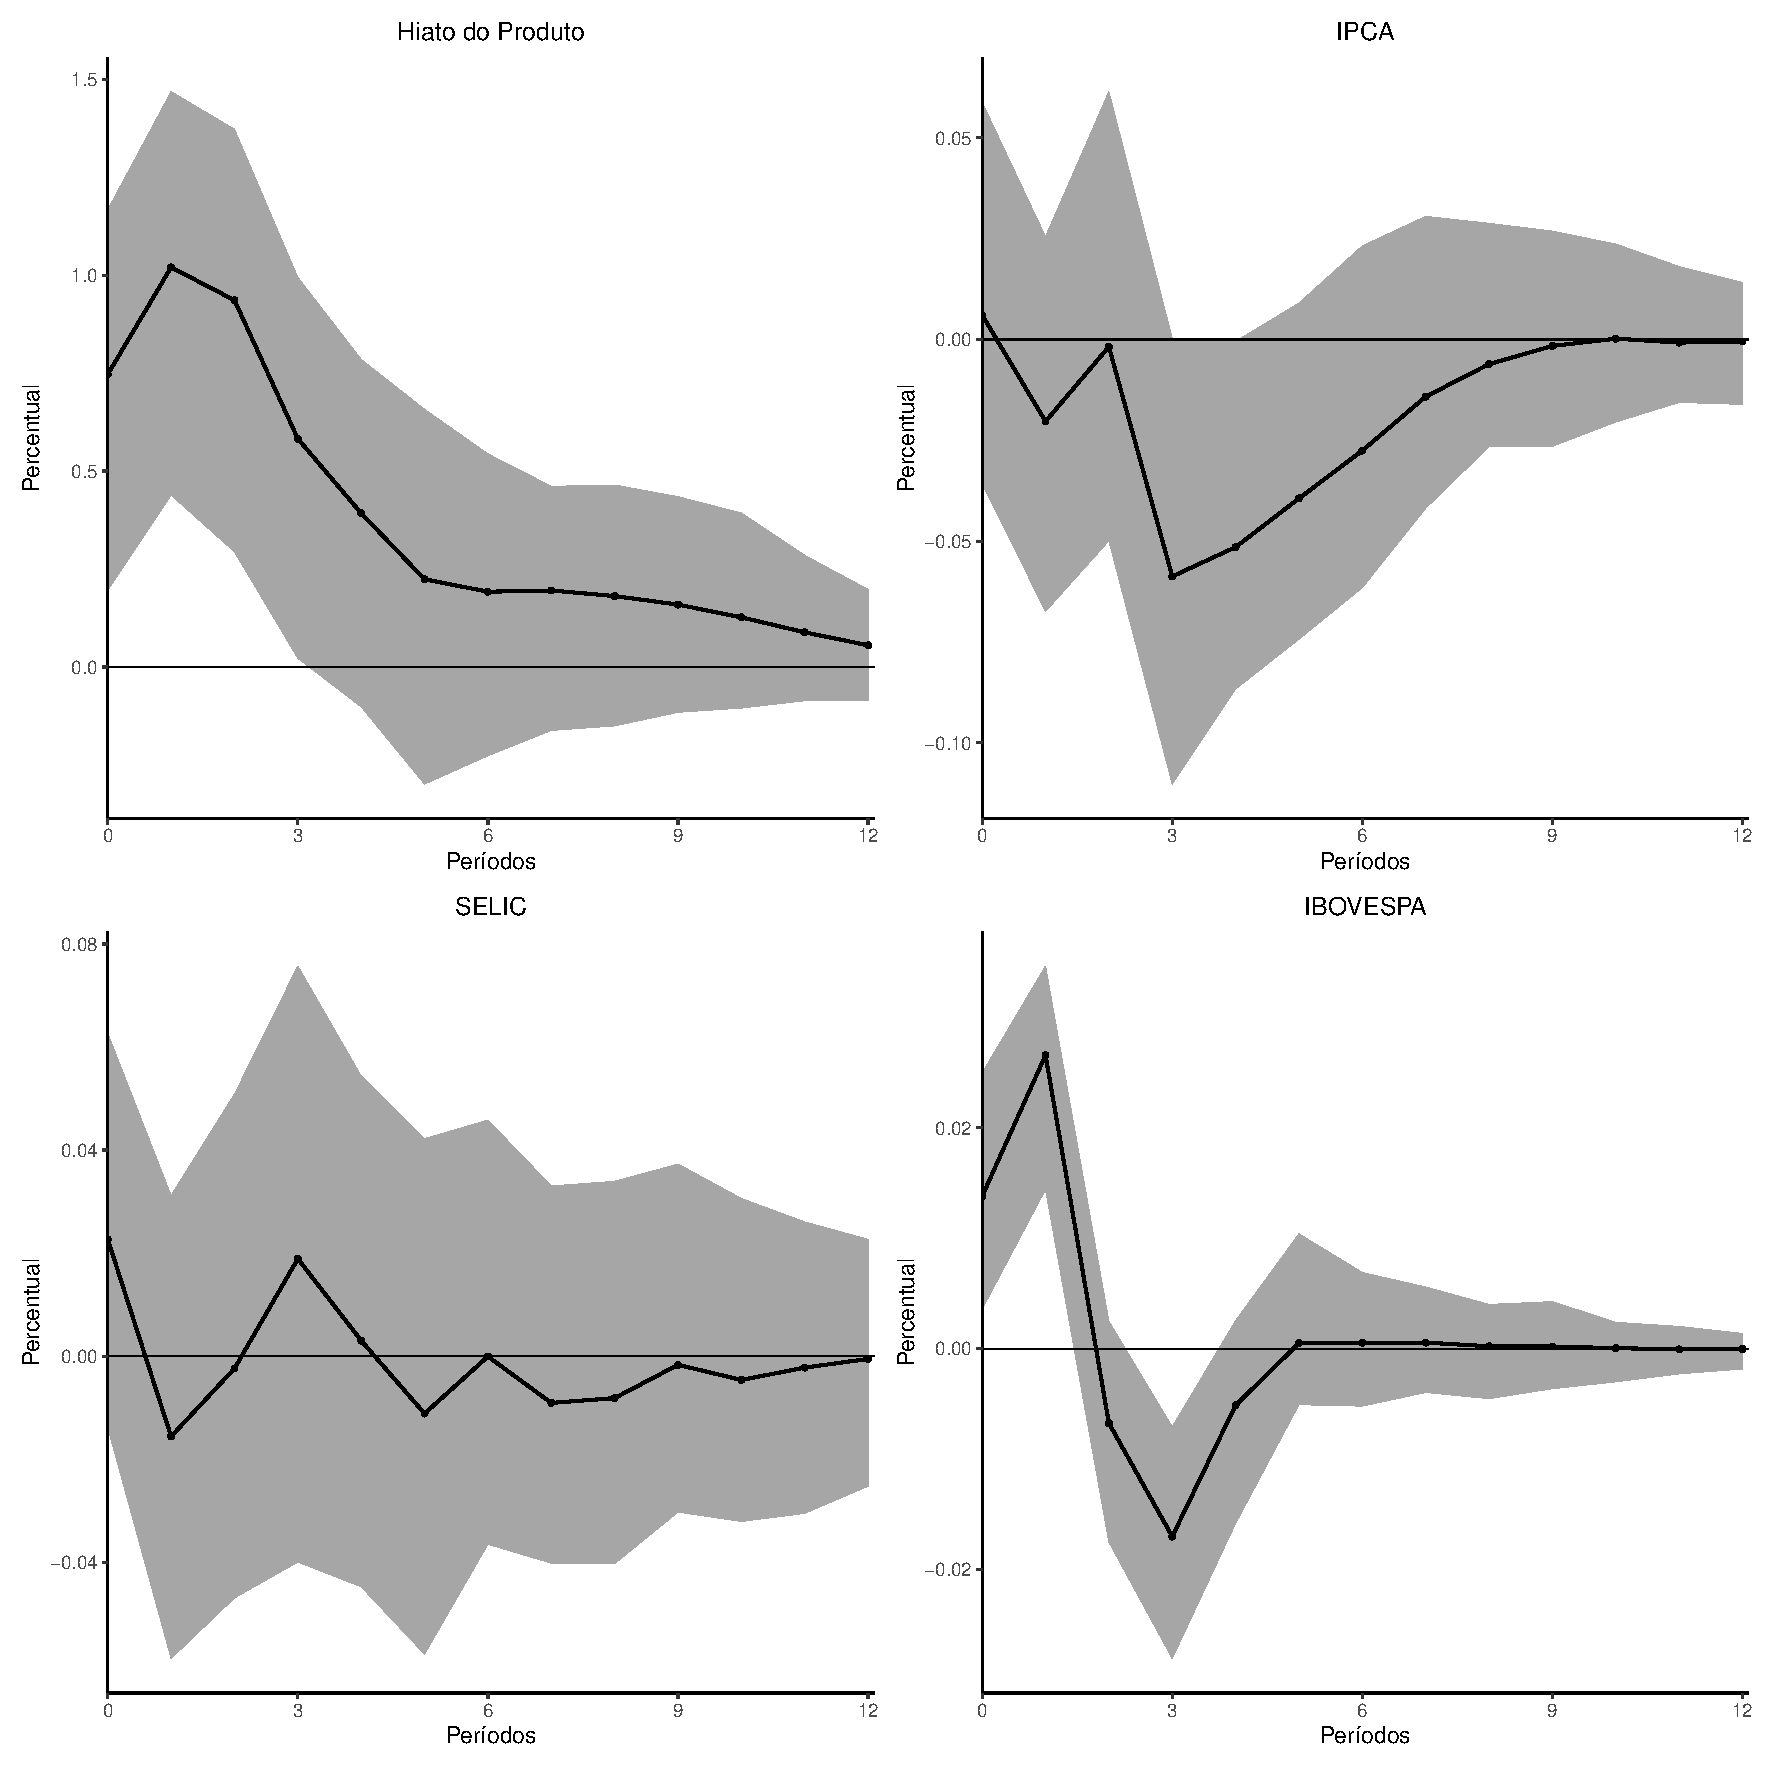
\includegraphics[width=0.85\textwidth]{imagens/irf_isv.pdf}
    \caption*{Fonte : Elaboração Própria}
\end{figure}

Como é visto na Figura \ref{fig: irf_isv}, o Hiato do Produto sofre um choque positivo e, apesar de decrescimento do 2º período e seguindo essa tendência pelos 12 períodos seguintes, a sua elevação se mantém positiva ao longo da série. Para o IPCA, o choque é negativo, com queda até o 3º período e logo em seguida retorna a crescer, diminuindo seu impacto até retornar ao seu estado inicial após 12 períodos. Enquanto a série da taxa SELIC adquire um comportamento muito volátil, oscilando entre altas e quedas, impossibilitando assim um veredito. Por fim, vemos, num primeiro momento, uma variação positiva no índice BOVESPA, com queda brusca até o 3º período e retornando ao seu patamar inicial após 5 períodos. 

\begin{figure}[!h]
\centering
\caption{Função de Resposta ao Impulso para o Modelo 2 - ISL}
\label{fig: irf_isl}
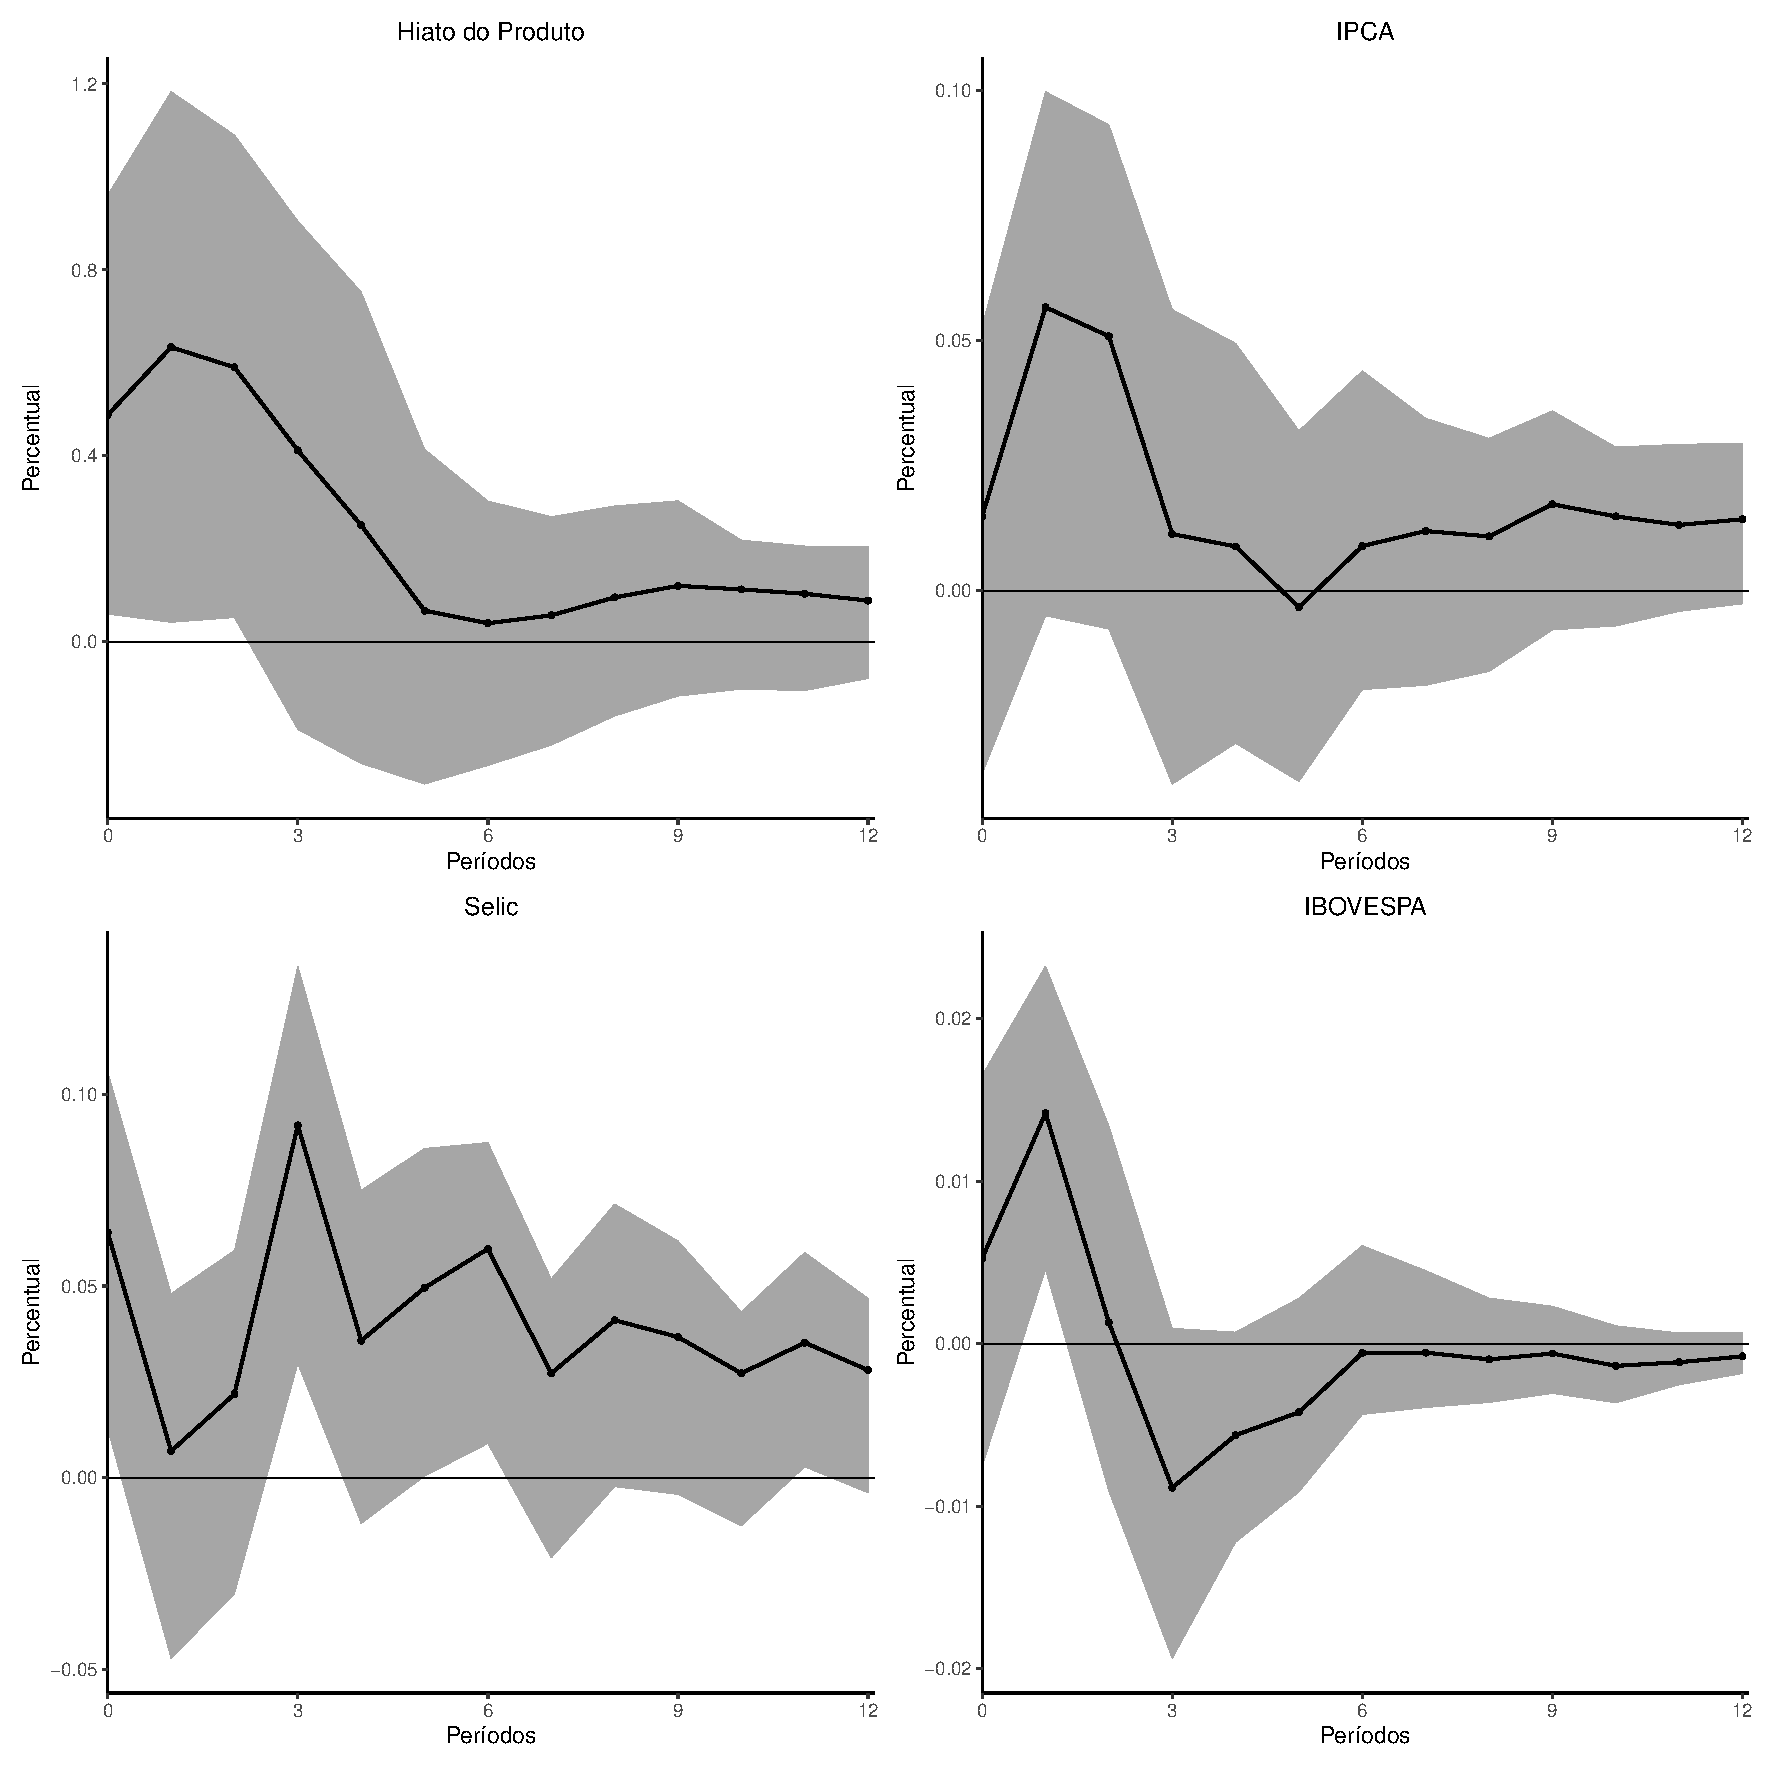
\includegraphics[width=0.85\textwidth]{imagens/irf_isl.pdf}
\caption*{Fonte : Elaboração Própria}
\end{figure}

Para o choque no índice LM, o comportamento é diferente em algumas séries. Apesar da semelhança do choque para o Hiato do Produto, o ISL provém respostas diferentes no IPCA e SELIC. Para o IPCA, o choque é positivo e crescente num 1º período e logo após o seu pico, ele torna a decrescer porém continuando positivo. Quanto a SELIC, embora seu nível oscile muito, a variação também é positiva ao longo dos períodos seguintes ao choque. Por último, o índice BOVESPA aparenta semelhança com o resultado do ISV, porém, seus resultados são predominantemente negativos, sem sinal de recuperação completa no horizonte de tempo.

Tais comportamentos fazem sentido à luz da economia, já que visto um choque positivo, a produção da economia tende a crescer, mensurado aqui pelo hiato, provocando uma elevação dos preços acompanhada pela subida da taxa de juros na tentativa de apaziguar o aumento dos preços. Por último, o comportamento da série dos retornos do BOVESPA podem ser explicados pelo cenário volátil e positivo para as séries de preços e taxa de juros, prejudicando assim seus desempenho no longo prazo.

Por fim, dadas as respostas ao choque vistas nas Figuras \ref{fig: irf_isv} e \ref{fig: irf_isl}, tais resultados corroboram a literatura econômica do assunto. Pois, como vemos, o índice VADER não provém tanta acurácia quanto o índice LM, visto que o primeiro não envolve as características e termos específicos ao campo econômico quanto o segundo. Tendo isso em vista, o índice LM-SA parece se adaptar melhor ao campo econômico do que o índice VADER por conta da sua fundamentação teórica econômica e nos retornar resultados mais contundentes à realidade.
